\renewcommand\labelenumi{(\roman{enumi})}
\renewcommand\theenumi\labelenumi

\chapter{Introduction}
\label{chapterIntro}
\chaptermark{Introduction}

Current society is facing a challenge to mitigate the effects of climate change. To keep global temperature rise below 2$^{\circ}$C stated in the Paris Agreement, the whole energy system is called to action: transform a mainly fossil-based electricity generation scenario into carbon-neutral, mostly based on renewable energy sources. The challenge is even more significant since it is expected that the electricity consumption will increase from 20\% to 40\% by 2050, according to \cite{IRENA2018}. This can be observed in Figure \ref{fig:scenarios}, where the scenario by 2050 expects 85\% of the electricity supply to be covered by renewables. 

\vspace*{3mm}
\begin{figure}[htbp]
	\centering 
	\includegraphics[width=0.9\columnwidth ]{ChapterIntro/Figures/scenarios2.pdf}
	   %\vspace*{-8cm}
		\caption{Renewable Energy Sources penetration scenario. Based on \cite{IRENA2018}}  
		\label{fig:scenarios}
\end{figure}
%\vspace*{1.5mm}
\newpage
This chapter aims to provide an overview of the current state of the electricity system and its agents to highlight the main shortcomings, challenges, and opportunities for implementing the energy transition roadmap. 

The following pages cover the main aspects related to the current scenario in the energy transition, such as the regulation related to distribution system operators and smart grids, the technical aspects of distributed energy resources and related technologies, the role of demand-side and end-user's awareness, and lastly the role of new business agents and services that can help distribution network operators to become key agents in the development of smart grids and achievement of the decarbonization objectives for 2050. 


\section{Smart Grids. The evolution of the electrical network}

%\subsection{Electricity network}
The physical infrastructure of the electricity network is composed by generators, transmission network, distribution network and end-users or consumers.

%, as shown in Figure \ref{fig:ree}. 
%
%\begin{figure}[htbp]
%	\centering 
%	\includegraphics[width=1\columnwidth ]{ChapterIntro/Figures/REE_english.pdf}
%	   %\vspace*{-8cm}
%		\caption{Electricity network scheme. Adapted from \cite{RedElectricadeEspana}}  
%		\label{fig:ree}
%\end{figure}

Generators are the main agents feeding the grid downstream. Large generators can produce a range from 6 kV to 20 kV \cite{Gomez-Exposito2008}, to then increase the voltage up to 200 kV in order to connect to the high voltage (HV) tramission lines. The transmission network is the responsible for the electricity transportation over long distances, and it is done at HV level. By doing this, the transmission losses are lower while using a cheaper infrastructure. The tranmission network voltage level usually ranges from 200 kV to 1000 kV \cite{Erbach2016}, and both generators and HV-MV transformers are the main elements connected to it. Due to their critical position in the system, connecting generation and consumption sides, transmission grids are meshed to avoid collapsing when there is any failure in on of the lines. On top of that, this layout allows the distribution of the loads through different tramission lines with the objective of reducing losses and avoiding congestions. Transmission networks are operated by the so-called Transmission System Operators (TSO). Similarly, distribution networks are responsible for the energy distribution and transportation for shorter distances. One could consider a distribution grid when its voltage levels are either medium-voltage (MV) and low-voltage (LV). By definition, the voltage levels considered for distribution networks are: 132 kV, 66 kV, 45 kV, 30 kV, 20 kV, 10 kV, 6 kV, 3 kV, 1 kV, 400 V and 230 V \cite{Gomez-Exposito2008, Erbach2016}. 

Differently as seen in the transmission system, the assets connected at distribution level are mainly loads ranging from industrial loads, connected at MV, to residential loads, most usually connected at the LV level. However, generation units can also be connected  at the distribution level, usually only considering renewable sources. The configuration layout of distribution networks is commonly not redundant, meaning that they do not usually use meshed configurations. As a result, these networks are not as redundant as the transmission system. Hence, this could lead to problems when DERs are connected to MV or LV connection points, leading to congestions  in distribution networks that were not expected when the network was implemented. Distribution networks are managed by Distribution System Operators (DSO), who connect consumers, install electricity meters and communicate the end-user consumption to energy suppliers or retailers \cite{Erbach2016}. An overview of the previously mentioned elements is shown in Figure \ref{fig:networkscheme}. 


\begin{figure}[htbp]
	\centering 
	\includegraphics[width=0.6\columnwidth ]{ChapterIntro/Figures/13.pdf}
	   %\vspace*{-8cm}
		\caption{Electricity network scheme}  
		\label{fig:networkscheme}
\end{figure}

%Extracted from \cite{Erbach2016}
%\subsection{Smart Grids}

Despite the scenarios where renewables are the main source for electricity production, it is a fact that geographical, economical and social-cultural barriers are still slowing down the implementation of renewable energy projects in some locations in the landfield \cite{ASANTE2020111479, barriers2020}, leading to newer technologies to allocate renewable sources in places where a larger power output can be obtained, and generally less concern by end-users in terms of environmental and visual impact of them, such as off-shore wind turbines \cite{Kaldellis2016, KPMG2019}, connected to the transmission network. At the same time, as electricity demand on grids increased due to the electrification of appliances, distribution system operators (DSOs) started to face congestions in their networks, and hence utilities started to find solutions for managing these peak loads, usually located in specific time periods.  This combined to the implementation of smart meters so utilities could encourage customers to switch consumption from peak to non-peak hours, and the need for monitoring and controlling the operation of the distribution network enhanced the development of smart grids.

Traditionally, electric power systems have been centralizsed structures organized into generation, transmission and distribution, placing end-users and the endpoint of the supply chain. This was an unidirectional structure where electricity generated by large power plants was transported by means of transmission and distribution networks, to be delivered to end-users. 

Furthermore, the emergence of the social awareness of the environmental impact of the end-users consumption, the increase of the electricity prices, as well as the emergence of the so-called distributed energy resources (DERs), such as small-scale PV installations (mainly rooftop), storage systems, electric vehicles (EVs) and smart home appliances are transforming the end-users into active participants in the power system. The increasing penetration of these decentralized resources, as well as the emergence of new market agents like prosumers, aggregators and active consumers, are pushing the electricity system to include innovation in their business models, creating the paradigm of smart grids. According to \cite{EuropeanParliamentSG}, smart grids can be defined as:
\vspace*{3mm}
\begin{tcolorbox}
\textit{"An electricity network that can integrate in a cost efficient manner the behaviour and actions of all users connected to it, including generators, consumers and those that both generate and consume, in order to ensure an economically efficient and sustainable power system with low losses and high levels of quality, security of supply and safety".} 
\end{tcolorbox}
\vspace*{5mm}

%\begin{figure}[htbp]
%	\centering 
%	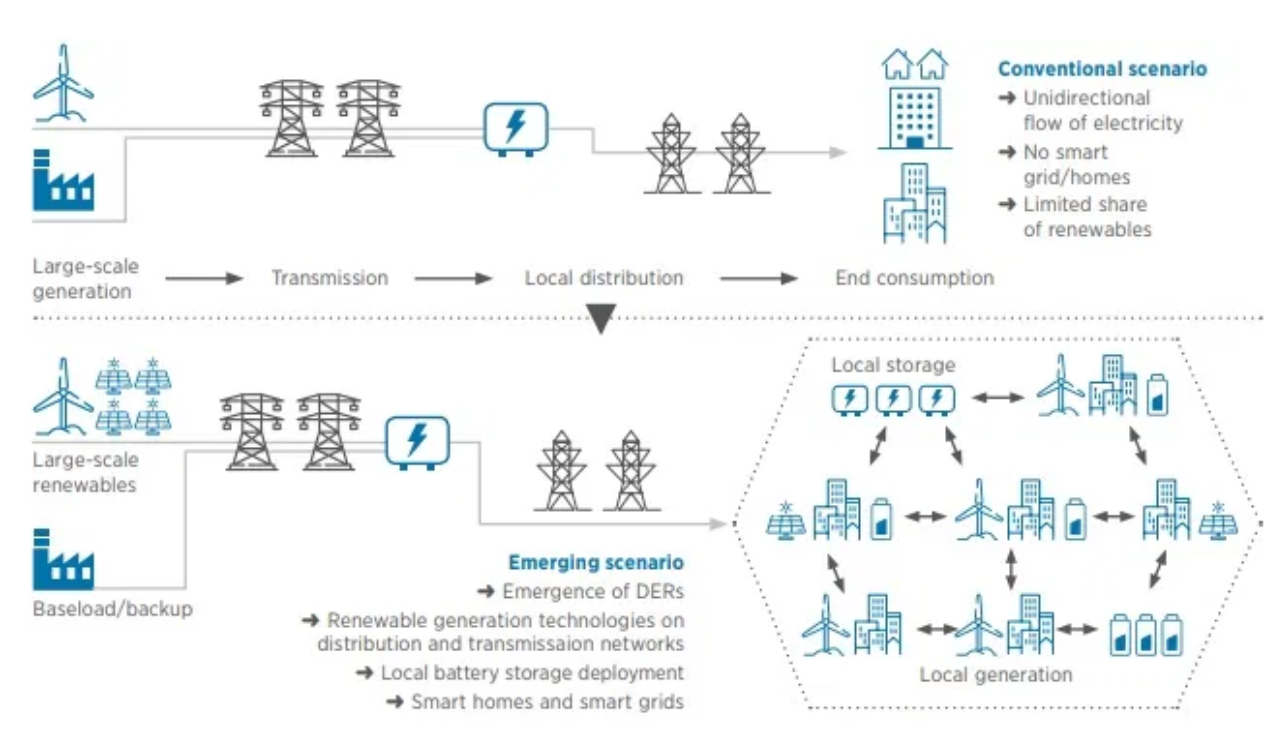
\includegraphics[width=0.9\columnwidth ]{ChapterIntro/Figures/Irena-DSO-1.png}
%	   %\vspace*{-8cm}
%		\caption{Conventional scenario vs Smart Grids. Extracted from \cite{IRENA2018}}  
%		\label{fig:IRENA-DSO}
%\end{figure}

However, it is not only in terms of technological innovation to fulfill the electricity transition roadmap. Changing the regulatory framework mainly for DSOs to adapt the current regulation for the operation of the distribution network to the new challenges placed by DERs is a key factor for the success of the energy transition.

With the liberalisation of the electricity markets all over Europe, due to the promotion of directives such as the ones in the First, Second and Third Energy packages \cite{EuropeanCommission2003, EuropeanCommission2009} to create a more robust internal market \cite{Hancher2017, EUPHEMIA2016, antonopoulos2020nodal}, grid planning faced problems related to generation forecast. Because at that point the generation at the HV side of the grid was not 100$\%$ planned anymore. However, the network overcame the problem establishing rules where these new agents must inform of their operations a centralised organisation in order to maintain the balance of the system, and creating a markets-system where TSOs upload their needs and generators their offers. 

Nowadays the EU is promoting another change in the structure of the electricity market, imposed by the need to decarbonise the energy sector by 2050 and the willingness to empower the citizen changing its role from pure consumer to a new agent in the market \cite{Hancher2017}. This is mainly going to be done by promoting the integration of DERs in the distribution grid which supposes an entirely new approach to the grid management. Challenges like reverse power flows and an increase of voltages near the point of coupling, among others, will arise. This structural change of the electricity system has been changing habits in the sector for some years now, and with these new ways to proceed challenges have arisen, from \cite{Bollen2011} the main changes can be classified as:

\begin{enumerate}
\item With the liberalization of the generation, system operators are less capable of limiting
connections of new generation assets which can drive the grid, at some locations, to its
limits.
\item Formerly traditional generators' location was determined considering the interests of the system
operator and the constraints related to the construction of such large power plants.
Nowadays, the location of new RES power plants is instead related to energy source availability.
\item RES generation tends to connect at distribution level instead of transmission level where
all the main generators were connected.
\item Democratization of generation assets which, other than the new cases stated above, can
transform traditional passive-customers to active customers and thus increase the variability
of the demand.

\end{enumerate}

These four changes in the power system structure can and will be an improvement in terms of clean generation, increased energy efficiency, customer empowerment, and grid reliability, among others. However, the truth is that nowadays most of the European grids are far from being ready to face such challenging opportunities and these new approaches are also making arise new problematic, and not-so-new ones, that can be divided into two main groups: 
\begin{enumerate}
\item \textbf{Generation and load balancing:} If there is no balance between generation and demand, the frequency of the system starts to deviate from the nominal value; this may be a problem for some electric/electronic loads. However, the main concern arises when large generators are synchronous machines. In an intense frequency deviation event some generators may trip from the grid, causing even a harder frequency deviation. This domino-like problematic is called cascade tripping and can lead to a local or even "global" system blackout. This problematic has been a concern for the system since its beginnings because the load forecast is not always accurate. However, large generator units can be mandatorily disconnected from the grid for safety purposes \cite{Bollen2011}. Then, the challenge increased with the liberalization of the generation market. Nowadays, with the introduction of DERs and the empowerment of the user via demand-modulation strategies, the future forecast of generation and demand is expected to be more challenging than ever.

\item \textbf{Distribution grid congestion:} Grid congestion, mainly at TSO level but also at DSO level,has always existed. However, due to the traditional operation of the grid, the fit-and forget approach consisting of investing in expanding the infrastructure was the most costefficient approach at the distribution level. With the uncontrolled connection, in terms of number but also location and characteristics, of new DER assets to medium and low voltage grids, a new grid structure may be needed from the fit-and-forget perspective. However, this does not seem either rational nor cost-effective viable, and instead, these new congestion challenges will need to be addressed from an active (real-time) management approach.
\end{enumerate}


\section{Regulation framework and new agents in the energy transition}
For the last 15 years global warming awareness and a more rational approach to production and consumption of goods and habits have been an increasing concern for societies with a firmly established welfare state. Related to this new approach, electricity markets have been the target of criticism due to their massive contribution to the emission of greenhouse effect gases \cite{Hancher2017}. Within the European energy policy context, the chosen way to carry out this reduction of emissions by the energy sector is enhancing a higher penetration of DERs (particularly RESs) in distribution networks. This positioning, while has multiple potential benefits for the grid and its agents, also sets out new challenges to be faced.
All the perks and disadvantages of a higher share of DERs need to be adequately regulated in order to keep secure the functioning and operation of the grid. It also has to be noted that inside the EU energy policies, the environmental concern is nowadaysone of the main drivers. However, there are also other key objectives to achieve, which in some cases will present synergies, but in other cases, could collide among them. 

The creation of the Winter Package the year 2016, also known as Clean Energy Package for all Europeans \cite{validzic2017clean}, started after the European Commission had evaluated the performance of the Third Energy Package established in 2009.  After assessing the outcomes of the previous energy packages, the objectives starting back then could be grouped in three, as follows: 
\begin{enumerate}
\item Adapting to the decentralization of the power system. 
\item Empowering customers and citizens. 
\item Ensuring the internal market level playing field. 
\end{enumerate}

The Clean Energy package is a set of regulations and directives published in June 2019 to promote the energy transition started with the Third Energy Package back in 2009. Among the CEP regulations and directives, the ones that address the electric sector are the e-Directive (EC 2019/944; \cite{Directive2019944}) and the e-Regulation (EC 2019/943; \cite{Directive2019943}), whose subject matter and scope is centred in \textit{"setting the basis for an efficient achievement of the objectives of the Energy Union and in particular the climate and energy framework for 2030"} (e-Regulation), \textit{"via the creation of common rules for all the assets connected to the power system, with a view to creating truly integrated, competitive, consumer-centred, flexible, fair and transparent electricity markets in the Union"} (e-Directive). The e-Directive and e-Regulation are mainly focused towards the creation of market models to
promote the energy transition. In terms of market design there is a group of markets, local energy and flexibility markets, that can be crucial to promote the widespread of new agents and technologies \cite{Xu2019}.


\section{Flexibility as a service for the energy transition}
Power system flexibility will play a key role in the energy transition and the next generation electric grid, and some of the main outcomes of implementing flexibility are the possibility to replace fossil fuel generators with clean and renewable energy sources; increase reliability and resilience against disruptive events; improve performance and reduce cost of new and existing assets and achieve the scenario where a low carbon economy is possible. 

In general terms, flexibility can be defined as follows, according to the International Smart Grid Action Network (ISGAN)\cite{Hillberg2019}.
\vspace*{3mm}
\begin{tcolorbox}
\textit{"The ability of a power system to reliably and cost-effectively manage the variability and uncertainty of demand and supply accross all relevant timescales."}
\end{tcolorbox} 
\vspace*{3mm}

Traditionally, these variations from the demand side have been overcome by means of fuel-based flexible large generators such as carbon and gas turbine; and pumped hydro power plants, which were forces to be able to provide flexibility. Those changes in the demand-side where mainly from changes in the load consumption based on consumer behavior.
Some of these requirements for large generators are still considered in the new regulation under the Clean Energy Package and Grid Codes \cite{validzic2017clean}. However, most of the requisites are not mandatory for smaller generator units, and with the new paradigm where there is a reduction in the number of synchronous generators and more difficulties to forecast demand and generation, the remanining generator units might not be able to handle the flexibility required to keep the grid consumption and generation balance. This will suppose an increased need for flexibility \cite{Xu2019}. Besides, the increasing penetration of DERs into the MV and LV grid will suppose some challenges in terms of network operation, which will need to be addressed by the DSOs by means of active management and flexibility activation to avoid grid reinforcement. For these reasons, flexibility markets are being recognized in the e-Directive \cite{Directive2019944} as a key element to support a safer and more efficient use of the already existing grids.
According to the same institution, flexibility will enable all stakeholder and elements of the grid considering generators, consumers/end-users, storage and infrastructure to be active participants in the energy system, also enabling the cost-efficient development of RES and more resilient power systems \cite{Hillberg2019}.  

\begin{figure}[h]
	\centering 
	\includegraphics[width=1\columnwidth ]{ChapterIntro/Figures/load_curve.pdf}
	   %\vspace*{-8cm}
		\caption{Evolution of the demand curve when implementing demand-side management or flexibility.}  
		\label{fig:load_shifting}
\end{figure}


Due to the increase of electricity consumption and DERs integration in the last 10 years, the consumer behavior patterns have been broadly studied \cite{ZHOU201773,TORRITI2014265}, showing that the electricity consumption is focused at specific time periods, such as noon and in the evening. With the implementation of DERs and the increase of the electricity consumption, there is a possibility to include flexibility in power systems by achieving the paradigm where consumption follows the generation curve only partially. That could lead to implement flexibility in the demand-side by shifting the consumption of some assets or the production of some small scale generators or storage systems to other time periods, as seen in Figure \ref{fig:load_shifting}. Demand-side flexibility can be defined as follows, according to \cite{EuropeanSmartGridsTaskForceExpertGroup32019}:  

\begin{tcolorbox}
\textit{"The ability of a customer or prosumer to deviate from its normal electricity consumption or production profile, in response to price signals or market incentives"} 
\end{tcolorbox}

Hence, demand-side flexibility can help developing smart grids and achieving the Paris Agreement objectives, by means of distributed energy resources, the change on their electricity consumption profile and the integration of energy storage and electric vehicles. 
%Demand-side flexibility is based on load, demand-side generation and demand-side storage. The Universal Smart Energy Framework (USEF) defined a wide range of services that could be provided to network operators, retailers, balancing parties thanks to demand-side flexibility under demand-side management. An overview of the flexibility products can be seen in Figure \ref{fig:DSF}. 
%
%\begin{figure}[h]
%	\centering 
%	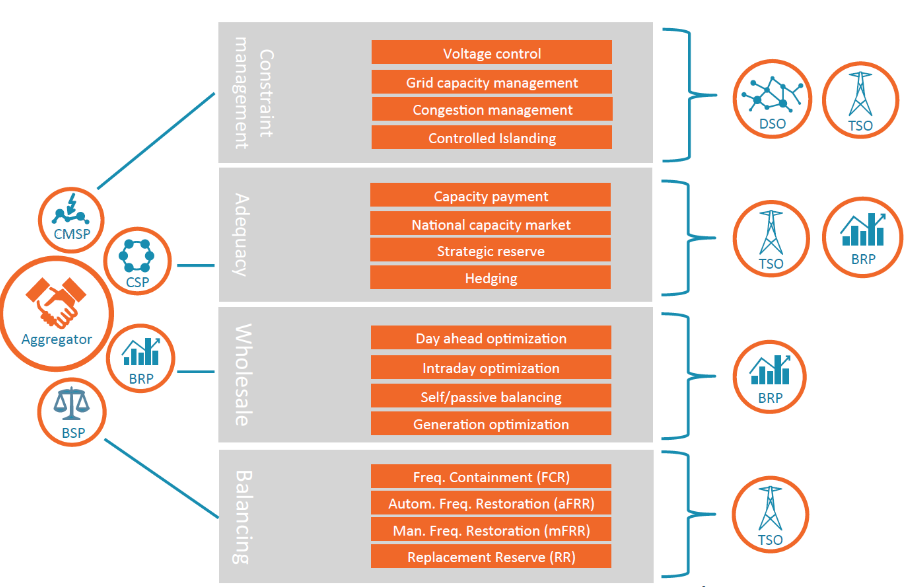
\includegraphics[width=1\columnwidth ]{ChapterIntro/Figures/USEF_DSF.png}
%	   %\vspace*{-8cm}
%		\caption{Products and services available from the demand-side. Extracted from \cite{USEFFoundation2015a}}  
%		\label{fig:DSF}
%\end{figure}


\section{Sustainability of smart grids and DERs}
Sustainability can be understood as a progress model that considers not only economic, but also environmental and society needs in order to develop an economic model that maintains an ecological balance. The 2030 Agenda for Sustainable Development, agreed by all United Nations Member States, defined 17 goals calling for action by all countries with the objective to achieve a sustainable and prosper future \cite{SDGOALS2015}. Many of the goals are aligned with the energy transition roadmap, and with the implementation of demand-side activities for encouraging end-users as market participants. Objectives 7, 11, 12 and 13 of the Sustainable Development Goals for 2030 (Figure \ref{fig:sdg}) are related to the previous statement, encouraging all Member States to include sustainability when planning the electricity system and market of the near-future.  

\begin{figure}[h]
	\centering 
	
\includegraphics[width=1\columnwidth ]{ChapterIntro/Figures/SDG.png}
	   %\vspace*{-8cm}
		\caption{Sustainable Development Goals defined by the United Nations.}  
		\label{fig:sdg}
\end{figure}    

The increase of renewable generation has provided and is providing many benefits in the road towards a decarbonized power system. However, in the past years, social concerns about the environmental impact of renewable technologies have arisen \cite{Temper2020}, with more than 3000 environmental conflicts based on renewable energy-related projects. These problems are based on the fact that these projects do not take into consideration neither the acceptance of the population living close to the renewable energy plant location, nor the consequences of having the power plant, such as the reduction of agriculture fields or the impact on the land prices. 


The decentralization of the renewable generation with the appearance of DERs has a large potential to succeed in the energy transition roadmap. However, sustainability must be taken into consideration in each and every step, even in local energy communities and DERs \cite{AMPONSAH2014461}.
% It can be seen as the intersection of the previously mentioned three concepts, as outlined in Figure \ref{fig:sust}.

Some of the current methodologies for calculating the environmental impact of renewable energy technologies assume that the carbon footprint of renewable sources is zero, because they only consider the CO$_2$ emission factor under the operation phase \cite{IRENA2020}. Renewable energy technologies, Electric vehicles and storage systems can be carbon neutral under the operation phase, but they are not zero, and their contribute negatively to other environmental indicators when considering the entire life cycle. There is a non-negligible carbon footprint or other environmental impacts such as water usage and polution and ozone contribution that must be considered \cite{en12214214, Moro2017, Jiang2018}. Furthermore, when developing smart grids and renewable energy sources and energy transition policies, a previous analysis should be performed in order to understand the current installed capacity in the country, in order to lower the environmental impact by implementing such technologies \cite{Treyer2014}.
%
%\begin{figure}[h]
%	\centering 
%	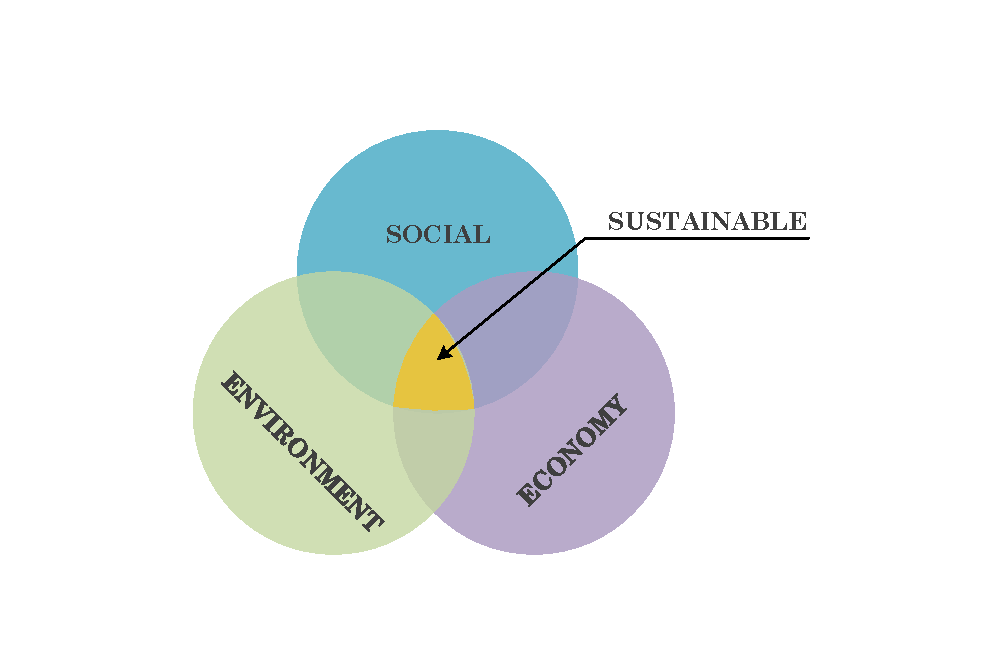
\includegraphics[width=0.7\columnwidth ]{ChapterIntro/Figures/SUSTAINABILITY.pdf}
%	   %\vspace*{-8cm}
%		\caption{Definition of sustainability.}  
%		\label{fig:sust}
%\end{figure}

Technologies and methodologies such as circular economy, second-life options for storage systems, and life-cycle assessment (LCA) are key to check the viability of renewable energy projects and smart grids implementation. More specifically, LCA is a powerful a tool for assessing environmental impacts of renewable energy sources, so as to assess the environmental impact based on indicators of renewable energy technologies and smart grids throughout the entire lifecyle. 



\newpage 
\section{Objectives and scope}
Several past and recent works in the literature have dealt with the development of smart grids and defining local electricity markets for enhancing the energy transition. The majority of these studies are based on DERs integration, optimization at household level and forecast of indivual assets. The majority of these studies consider flexibility as a known signal, assuming a perfect forecast and a direct control of the flexible assets, as a way of simplifying the operation of the local flexibility markets. Furthermore, they assume that both the aggregator and the DSO share information regarding the flexible assets or the network layout, or can even control the flexible assets or the network. The fact is that, in reality, and according to the current regulation, they must be different entities, and as a result they might differ in the business model. Furthemore, even though there is a significant amount of data being collected at different points of the power system thanks to smart meters rolling out and more ICT installed, there is still a difficulty to get access to this data. As a result, the access to data is still a challenge for smart grids agents to develop innovative algorithms and solution for the energy transition era. Combining the previous facts and challenges, the main research question that this thesis aims to answer is the following one:

\vspace*{1mm}
\begin{tcolorbox}
What are the possibilities to develop and activate flexibility in distribution networks, by engaging demand-side and ensuring that the sustainability goals are taken into consideration, considering data-driven approaches and challenges? 
\end{tcolorbox}

This can be considered a broad question, and hence the knowledge barriers should be found in order to establish the baseline for the PhD research. This manuscript aims to answer this question focusing on the role of the demand side and their flexible assets and what the benefits and consequences would be for distribution networks, managed by DSOs. Figure \ref{fig:objectives} provides an overview of the system under study, considering the demand-side by means of prosumers and flexible assets; the aggregator as the entity that collects all the available flexibility and provides this service to the DSO by controlling the end-user's assets; the DSO as the main client of this flexibility; the electricity market to understand which role plays the flexibility in a market-environment; and lastly the environment, to assess the global warming potential and other environmental impacts that flexibility could reduce or increase. Based on the previous discussion, more specific objectives can be outlined in order to set the basis for the research developed in this thesis. The research questions that led to the objectives of the thesis are outlined below: 

\begin{tcolorbox}
\begin{enumerate}
\item What are the possible market schemes to integrate DERs and demand-side management, while at the same time ensuring that network operators can benefit from these services?  
\item How can flexibility be defined and modeled, based on the final users providing and using this flexibility, as well as the time horizon purposes? 
\item How can flexibility be forecast, from the aggregator point of view, with very limited amount of data available, in a fast and reliable approach so as to know in advance the flexibility available in the portfolio, in order to provide flexibility to DSOs for operation purposes?
\item How can this flexibility help DSOs to mitigate or avoid congestions in MV networks, and how can this flexibility request be calculated so as to be economically better than investing in network expansion or hosting capacity?
\item How this scenario of flexibility provision can be environmentally assessed, so as to know if these approaches can be included in each and every country? Should the current installed capacity and generation portfolio be taken into account before the deployment of flexibility services in smart grids?
\end{enumerate}
\end{tcolorbox}

A conceptual overview of the different objectives outlined above is shown in Figure \ref{fig:objectives}, which can be also understood and the steps taken in this thesis. Each of the questions and objectives can be detailed and related to each of the chapters of this manuscript, as follows: 

\begin{enumerate}
\item \textbf{Analysis of the market schemes for energy and flexibility for the development of smart grids.} The first step of the thesis has the objective of defining the framework where new products and services can be implemented, with the purpose of providing smart grids stakeholders such as retailers, network operators and end-users a set of benefits. Special focus is set in energy and flexibility services for balancing agents and distribution network operators, with the creation of new market agents like the aggregator and the local market operators. Different market mechanisms for providing these services are analyzed, considering peer-to-peer and peer-to-platform approaches. 
\item \textbf{Definition of flexibility based on the main stakeholder, time horizon and business objective.} As a result of the previous state-of-the-art analysis, the research is focused on flexibility for the distribution network operator. The main research gap to address here is that distribution network operators require flexibility for the network operation, however current research still lacks a common definition for flexibility, and how can this flexibility be formulated based on the final user and the final approach of this flexibility. There are several differences to be considered if this flexibility is implemented for operation purposes or planning purposes. In this case, the role of the aggregator, the information exchange between these two agents as well as the regulation behind them are key for the development of successful flexibility services for the DSO.  
\item \textbf{Modeling and forecasting flexibility of an aggregator's portfolio based on statistical techniques.} Based on the result of the previous objective, a modeling and forecasting approach is developed under this objective of the PhD research. This methodology is based on a bottom up approach for collecting the flexible assets' submetering data, and later a hierarchical approach is performed with the approach to estimate the available flexibility in a two-level hierarchy. The underlying forecasting technique is based on statistical learning, considering several approaches. The benchmark model is defined by means of a particular case of the moving average, known as climatology model; and also considers the simple exponential smoothing. The more complex methodologies for forecasting the flexibility value is based on a conditional approach, and implementing probabilistic forecast by means of kernel density estimation and recursive maximum likelihood. This methodology is later implemented to a case study of an aggregator's portfolio to assess the goodness of fit. 
\item \textbf{Development of an optimization algorithm for the distribution network operation under congestion management scenarios.} Once the flexibility has been forecast by the aggregator, this service can be provided to the DSO for the correct operation of the distribution network. The research performed under this objective aims to provide DSOs with a tool to calculate the flexibility required for avoiding a congestion in the distribution network. This is implemented by means of an AC-OPF algorithm, with the main objective function of minimizing the flexibility activation costs that the aggregator should pay for it. The final purpose of activating flexibility in distribution networks is for DSOs to avoid the reinforcement of the network and activate flexibility instead. 
\item \textbf{Analysis of the environmental impact of the current electricity market generation scheme and evaluation of environmental savings by implementing flexibility.} The final step of the research aims to assess the whole idea and approach by evaluating potential savings in terms of CO$_2$ emissions in the generation profiles, based on a cradle-to-gate life cycle assessment methododology. This study defines a peak hourly LCA approach to highlight those time periods where flexibility could be activated and evaluate the environmental impact of these time periods. This methodology is implemented in five case studies in Europe to assess whether there are environmental savings or not. This approach can help policy makers to implement smart grids and energy transition initiatives not focusing only on the technical development, but also in terms of sustainability. 
\end{enumerate} 

\begin{figure}[h]
	\centering 
	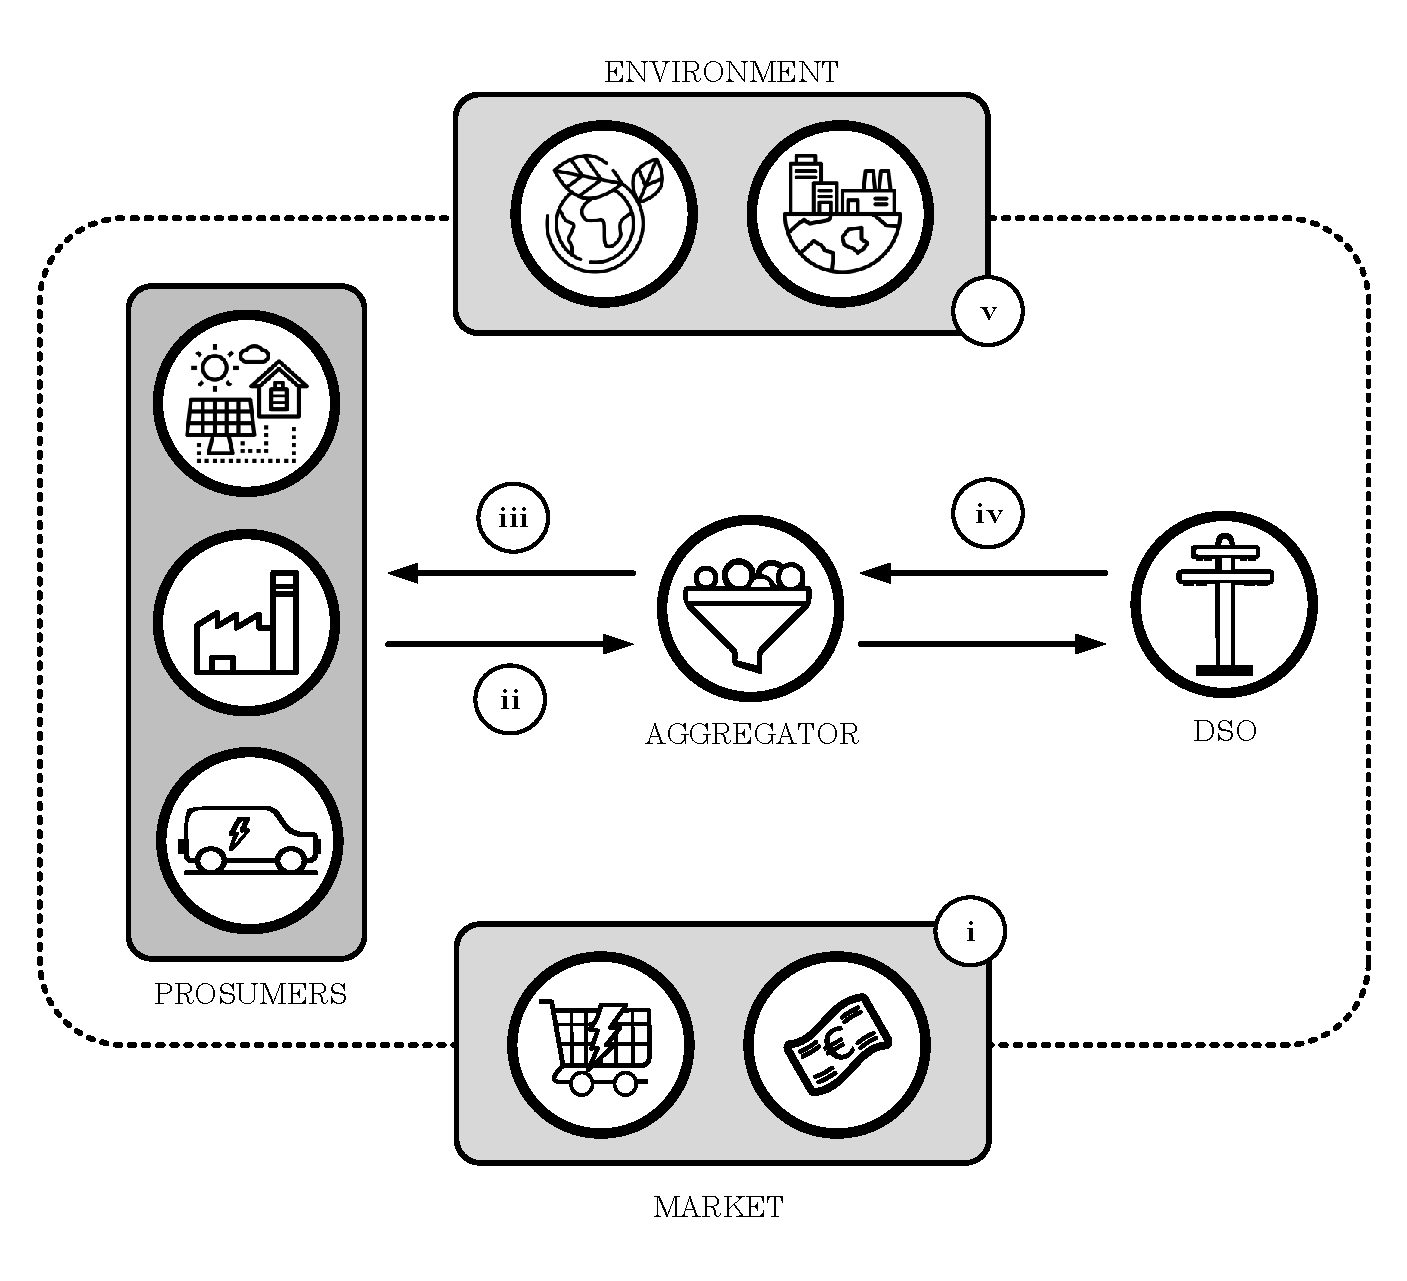
\includegraphics[width=0.75\columnwidth ]{ChapterIntro/Figures/objectives_figure_2.pdf}
	   %\vspace*{-8cm}
		\caption{Overview of the thesis objectives}  
		\label{fig:objectives}
\end{figure}



\newpage 
\section{Thesis related work and activities}
This section provides a summary of the work and the relevant activities that the author has participated in during the developlment of the thesis presented in this manuscpript. 
 	
Doctoral activities started in June 2017 with the collaboration on behalf of the EMPOWER \textit{Local electricity retail markets for prosumer smart grid power services } Project (Grant Agreement No. 646476). This work consisted on a review of the current state of the art in terms of Life Cycle Assessment Methodology in the field of smart grids, the understanding of how this methodology can be implemented in power systems and renewable energy technologies and the assessment of the environmental impact of the pilot-sites implemented throughout the project. This research resulted in a presentation in the General Assembly of the H2020 Project [P1] and the technical report [R2]. The research on the environmental assessment of ICT and Smart grids continued in the H2020 Project INVADE \textit{Integrated electric vehicles and batteries to empower distributed and centralised storage in distribution grids} (Grant Agreement No. 731148), in years  2018 and 2019, with the assessment of the environmental impact of electricity generation and the possibility of including flexibility to lower the environmental impact of electricity production in the INVADE pilot-sites. This research was performed in collaboration with the Finnish research center VTT, NTNU, Elaad and eSmart resulted in the journal publication [J1], a conference proceeding [C2], and technical reports [R3], [R5]. Dissemination events for the exploitation of the results took place in years 2019 and 2020, [P5] and [P11]. 

Since the main objective of the thesis is how new local markets and new service can help the deployment of smart grids, a thorough review of the state-of-the-art on local electricity market was done as a starting point of the doctoral research in 2018. This research was mainly focused on describing the basics on power systems and market mechanisms, as well as a literature review on local and micro-markets. As a result of that, a technical report was developed [R1], and two book chapters were published by Wiley ([B1],[B2]).  The evolution of this state-of-the-art review, combined with the collaboration with colleagues at CITCEA-UPC and other research centers and companies such as EYPESA and Smart Innovation Norway or on behalf the INVADE Project led to several outcomes covering from technical reports [T4], journal articles [J4] adnd [J5]; conference papers [C1], [C3] and [C4]; and presentations in local and international events [P3] and [P4].  

The evolution and implementation of smart grids based on data-driven approaches has been of interest of the author, and combined with collaboration with other universities as KU Leuven, DTU and KTH Stockholm on behalf of EIT InnoEnergy, resulted in [P6], [P10] and [P14]. 

%Escriure BD4OPEM aquí 
Year 2020 started with the kick-off the BD4OPEM H2020 Project \textit{Big Data for Open Innovation Energy Marketplace} (Grant Agreement No. 872525), with the participation of 12 partners from 8 different countries, and 5 pilot-sites. The research consisted on the development of algorithms for flexibility forecast and distribution network congestion management based on optimization techniques and flexibility provision. This work was combined with the Technical University of Denmark (DTU) under the external stay of the author, and in collaboration with other research centers and companies such as JSI and ICOM. This work resulted in a technical report [R6], two dissemination events [P12], [P15], and three journal publications under review or preparation [J2], [J3] and [J7].  

The international placement took place from March 2020 until April 2021, at the Electricity Markets (ELMA), DTU, Kongens Lyngby, Denmark. The topic was aggregated flexibility forecast based on probabilistic forecast techniques. It resulted in a journal paper [J2], and the database publication [D1]. During this period, the author has collaborated with KU Leuven in the core of the Data Science Working Group, with the aim of improving the knowledge of undergraduate students in the field of data science in the energy sector. This resulted in the publications [J6] and [J8]. 

%Since the author and the research center where the thesis was involved has a flair for knowledge transfer and higher and professional education, t
The author has collaborated with other entities and other researchers, resulting in the respective outcomes, which are not included in the thesis manuscript. This is the case of the collaboration with EIT InnoEnergy, whose core activity is the connection and cooperation between industry, universities, and research centers to reduce the gap between research and the market. In years 2018, 2019 and 2020 the author has been the lead teacher of the course on Control and Automation for the Efficient Use of Energy, developing the open-source learning material, and developing a course based on project-based learning and flipped classroom approach. This resulted in [E1] learning material, and dissemination of the results in different local conferences [P2], [P7] and [P8]. The project Learning Analytics started in September 2018, with the objective of monitoring students' performance to assess their engagement in the course, in collaboration with the Data Collection company DataLemon. This collaboration led to dissemination event [P9] and [P13], as well as an ongoing journal paper to be submitted in the near future. Other collaborations within the Electrical Engineering Department led to two outcomes: a MOOC course for wearable technology [E2], and a publication in a local journal [C5]. 


%\newpage 
\section{Thesis outline}
The content of the thesis is organized in the following chapters as follows:
\begin{itemize}
\item \textbf{Chapter 2} presents the overall state-of-the-art in terms of local energy markets, in order to define the role of flexibility in a local market and to which extent this service can help energy transition, and more specifically, DSOs. This work correspond to the first objective of the thesis \textit{(i)}. 
\item \textbf{Chapter 3} outlines how flexibility can be formulated, defined and modelled according to different approaches in terms of end-user, approach and time-horizon, covering the second objective of the thesis, providing different formulations for modeling flexibility \textit{(ii)}. 
\item \textbf{Chapter 4} presents the aggregated flexibility forecast for estimating the available flexibility within an aggregator's portfolio, with limited amount of information, for operation purposes and trading in a market or a bilateral contract. This chapter aims to fulfill the thirds approach of the thesis \textit{(iii)}. This formulation is implemented under a case study covering a portfolio of flexible assets such as Electric Vehicles, Space heaters and electric water boilers.  
\item \textbf{Chapter 5} outlines the AC-OPF formulation for calculating the flexibility requests needed by DSOs to solve congestions in MV networks by means of flexibility activation. This chapter corresponds to the fourth objective of the thesis research \textit{(iv)}.  
\item \textbf{Chapter 6} extends the scope of the previous research assessing the potential role of flexibility in different countries, in terms of sustainability. This chapter calculates the peak-hour environmental impact measured in CO$_2$ emissions, so as to establish a baseline for countries to understand where DERs and flexibility could be implemented and leading to a lower carbon footprint. This chapter focuses on the last objective of the research \textit{(v)}. 
\item \textbf{Appendix A} enumerates the publication and research outcomes both related and non-related to the thesis manuscript. 
\end{itemize}


